\documentclass[a4paper,10pt,table]{article}

\usepackage[left=3cm,top=2cm,right=3cm,bottom=3cm,nohead]{geometry} %
\usepackage[utf8]{inputenc}
\usepackage{polski}
\usepackage{pbox}
\usepackage[table,xcdraw]{xcolor}

\usepackage{multirow}

\usepackage{tabularx}

\usepackage{amsmath}
\usepackage{pdfpages}
\usepackage{hyperref}

\usepackage{pgfplots}

\usepackage{placeins}

\usepackage{pgf}
\usepackage{tikz}
\usepackage{caption}
\usepackage{subfigure}
\usepackage{multicol}
\usepackage{color} %red, green, blue, yellow, cyan, magenta, black, white
\definecolor{mygreen}{RGB}{28,172,0} % color values Red, Green, Blue
\definecolor{mylilas}{RGB}{170,55,241}
\usepackage{listings}
\usepackage{amssymb}
\usepackage{graphicx}

\newtheorem{twr}{Twierdzenie}

\lstdefinestyle{BashInputStyle}{
  language=bash,
  basicstyle=\small\sffamily,
  numbers=left,
  numberstyle=\tiny,
  numbersep=3pt,
  frame=tb,
  columns=fullflexible,
  backgroundcolor=\color{gray!20},
  linewidth=0.9\linewidth,
  xleftmargin=0.1\linewidth
}

\makeatletter
\newcommand{\lstuppercase}{\uppercase\expandafter{\expandafter\lst@token
                           \expandafter{\the\lst@token}}}
\newcommand{\lstlowercase}{\lowercase\expandafter{\expandafter\lst@token
                           \expandafter{\the\lst@token}}}
\makeatother

\lstdefinestyle{Oracle}{basicstyle=\ttfamily,
                        keywordstyle=\lstuppercase,
                        emphstyle=\itshape,
                        showstringspaces=false,
                        }
\lstdefinelanguage[Oracle]{SQL}[]{SQL}{
  morekeywords={ACCESS, MOD, NLS_DATE_FORMAT, NVL, REPLACE, SYSDATE,
                TO_CHAR, TO_NUMBER, TRUNC},
}
\definecolor{light-gray}{gray}{0.95}

\lstset{
  breaklines=true,                                     % line wrapping on
  language=SQL,
  frame=ltrb,
  framesep=5pt,
  basicstyle=\normalsize,
  keywordstyle=\ttfamily\color{green},
  identifierstyle=\ttfamily\color{blue}\bfseries,
  commentstyle=\color{Brown},
  stringstyle=\ttfamily,
  showstringspaces=ture,
  backgroundcolor=\color{light-gray},
  numbers=left
  }
  
  \lstset{language=Matlab,%
    %basicstyle=\color{red},
    breaklines=true,%
    morekeywords={matlab2tikz},
    keywordstyle=\color{blue},%
    morekeywords=[2]{1}, keywordstyle=[2]{\color{black}},
    identifierstyle=\color{black},%
    stringstyle=\color{mylilas},
    commentstyle=\color{mygreen},%
    showstringspaces=false,%without this there will be a symbol in the places where there is a space
    numbers=left,%
    numberstyle={\tiny \color{black}},% size of the numbers
    numbersep=9pt, % this defines how far the numbers are from the text
    emph=[1]{for,end,break},emphstyle=[1]\color{red}, %some words to emphasise
    %emph=[2]{word1,word2}, emphstyle=[2]{style},    
}




\begin{document}
% \renewcommand{\arraystretch}{1.8}
% \renewcommand{\arraystretch}{1.8}

\begin{titlepage}

\newcommand{\HRule}{\rule{\linewidth}{0.5mm}} % Defines a new command for the horizontal lines, change thickness here

\center % Center everything on the page
 
%----------------------------------------------------------------------------------------
%	HEADING SECTIONS
%----------------------------------------------------------------------------------------

\begin{center}

\includegraphics[scale=0.5]{agh.JPG}
\end{center}
\vspace*{10mm}
\textsc{\LARGE Akademia Górniczo-Hutnicza}\\[1.5cm] % Name of your university/college
\textsc{\Large Wydział Fizyki i Informatyki Stosowanej}\\[0.5cm] % Major heading such as course name
\textsc{\large Eksploracja Danych}\\[0.5cm] % Minor heading such as course title

%----------------------------------------------------------------------------------------
%	TITLE SECTION
%----------------------------------------------------------------------------------------

\HRule \\[0.4cm]
{ \Large \bfseries 
Szybka	klasteryzacja oparta o	maksima	gęstości}\\[0.4cm] % Title of your document
\HRule \\[1.5cm]
 
%----------------------------------------------------------------------------------------
%	AUTHOR SECTION
%----------------------------------------------------------------------------------------

\begin{minipage}{0.4\textwidth}
\begin{flushleft} \large
\emph{Autorzy:}\\
Maciej Kubicki\\
Tomasz Chronowski\\
\end{flushleft}
\end{minipage}
~
\begin{minipage}{0.4\textwidth}
\begin{flushright} \large
\emph{Prowadzący:} \\
dr inż. Szymon Łukasik
\end{flushright}
\end{minipage}\\[4cm]

% If you don't want a supervisor, uncomment the two lines below and remove the section above
%\Large \emph{Author:}\\
%John \textsc{Smith}\\[3cm] % Your name

%----------------------------------------------------------------------------------------
%	DATE SECTION
%----------------------------------------------------------------------------------------

{\large \today}\\[3cm] % Date, change the \today to a set date if you want to be precise

%----------------------------------------------------------------------------------------
%	LOGO SECTION
%----------------------------------------------------------------------------------------

%\includegraphics{Logo}\\[1cm] % Include a department/university logo - this will require the graphicx package
 
%----------------------------------------------------------------------------------------

\vfill % Fill the rest of the page with whitespace


\end{titlepage}
\newpage
\tableofcontents
\newpage
%------------------------------1-------------------------------

\section{Wstęp}
\subsection{Temat projektu}
Tematem naszego była implementacja algorytmu szybkiej klasteryzacji opartej o maksima gęstości z usprawnieniem w liczeniu odległości. Algorytm był przedstawiony w artykule autorów Rodriguez`a i	Laio`a pod tytułem	"Clustering	by	 fast	search	and	 find	of	density	peaks" w magazynie Science z	2015.
\subsection{Wykorzystane technologie i oprogramowanie}
Projekt został zrealizowany w Visual Studio 2017. Algorytm został zrealizowany w C++ z wykorzystaniem technologii MPI i OpenMP. Zgodnie z założeniami użyta została biblioteka FLANN. Pierwotnie chcieliśmy skorzystać z technologii CUDA(to prawdopodobnie przyśpieszyłoby algorytm znacząco), jednak kompilator z nowego VS nie poradził sobie z budową części biblioteki FLANN odpowiedzialnej za przerzucanie obliczeń na kartę graficzną. W każdym razie w kodzie w komentarzach umieściliśmy odpowiednie przykłady jakby to zostało zrealizowane.
\subsection{Repozytorium}
Adres repozytorium:\newline
\url{https://github.com/maciekkubicki/DenesityPeaksBasedClustering}

\newpage
\section{Implementacja}
Sama struktura programu jest oparta o MPI. Algorytm działa niezależnie od rozmiaru "świata". W funkcji \textbf{main} na początku deklarujemy środowisko MPI. Następnie sprawdzane są parametry z jakimi uruchomiono program - ilość oraz odpowiedniość. Następnie jeśli są odpowiednie to te parametry są przekazane do funkcji dokonującej klasteryzacji - \textbf{clustering}.
Lista parametrów:
\begin{itemize}
\item  \textbf{fileName} - nazwa plik z danymi do klasteryzacji, 
\item \textbf{radius} - rozmiar sąsiedztwa "punktu", 
\item \textbf{minDistF} - minimalna odległość "punktu" od innego "punktu" o większej gęstości, po to, by "punkt" był środkiem klastra (musi być spełniony warunek niżej), 
\item \textbf{minDensF} - minimalna gęstość "punktu", po to, by "punkt" był środkiem klastra (musi być spełniony warunek wyżej),
\item \textbf{excludeHalo = false} (opcjonalny) - wartość logiczna czy pominąć tzw. "punkty halo", 
\item \textbf{densCol = R} (opcjonalny)- "punkty halo" będą wykluczane na podstawie gęstości globalnej (gęstość sąsiedztwa bez brania pod uwagi do jakiego klastra należy sąsiad - enum = R = 1), lub też lokalnej(gęstość sąsiedztwa składająca się tylko z sąsiadów tego samego klastra co badany punkt - enum = CR = 4),
\item \textbf{factor = 1.f} (opcjonalny) - "punkty halo" są identyfikowane jeśli ich gęstość(globalna/lokalna) jest mniejsza, niż największa gęstość w obszarze brzegowym(w sąsiedztwie "punktu" brzegowego są "punkt/y" z innego/innych klastrów). Parametr \textbf{factor} dzieli tą największą gęstość, jest użyteczny w przypadku korzystanie z gęstości globalnej. 
\end{itemize}

Funkcja \textbf{clustering} jest przystosowana do działania równolegle. Proces o indeksie 0 wczytuje dane do macierzy i liczy maksymalną możliwą odległość między dwoma "punktami". Proces 0 dzieli dane między wszystkie procesy w "świecie" - użycie \textbf{broadcast} i \textbf{scatter}. W pierwszym kroku każdy proces znajduje gęstość sąsiedztwa przydzielonych mu "punktów" - \textbf{radiusSearch} z biblioteki FLANN. Następnie obliczone gęstości są porozsyłane do wszystkich procesów - \textbf{all\_gather}. W kolejnym kroku posiadając gęstości procesy znajdują odległości do punktów o większej gęstości, przechowujemy również indeks najbliższego sąsiada z większą gęstością - to ułatwi klasteryzację. Tu używamy \textbf{knnSearch} z FLANN(zgodnie z dokumentacjom projekt jest kompilowany z OpenMP i do przekazujemy do tej funkcji parametr z atrybutem \textbf{cores} równym 0, więc wyszukiwanie jest realizowane przy największej liczbie dostępnych rdzeni). W przypadku, gdy nie ma "punktu" o większej gęstości przypisana zostanie wartość maksymalnej możliwej odległości między punktami(znaleziona na początku). Dodatkowo może się zdarzyć, że w sąsiedztwie będzie kilka "punktów" o maksymalnej gęstości - jeśli to się stanie to naprawiamy to funkcjom \textbf{fix2}, której działanie przydałoby się usprawnić. Następnie znalezione odległości są normalizowane, by znajdowały się w przedziale $<0,1>$ i ustalane są środki klastrów na podstawie parametrów \textbf{minDistF} i \textbf{minDensF}. Sama klasteryzacja realizowana jest w miejscu przy pomocy funkcji rekurencyjnej - "punkt" jest przypisany do tego samego klastra co jego najbliższy sąsiad o większej gęstości. Następnie, jeśli wartość parametru \textbf{excludeHalo} jest prawdą to realizujemy pozbywanie się tych "punktów" z wykorzystaniem zadanego rodzaju gęstości i wielkościom parametru \textbf{factor}. Tu również używana jest funkcja \textbf{radiusSearch} z FLANN. Następnie dane są zebrane przy pomocy \textbf{all\_gather} i proces 0 zapisuje dane do pliku \textbf{outputp.dat}. 
\newpage
\section{Użycie}
Do przedstawienie algorytmu przygotowaliśmy kilka przykładowych zbirów danych, część jest wygenerowanych przez nas, a część z Internetu. Przykładowe komendy uruchomienia algorytmu wraz z parametrami znajdują się w pliku \textbf{readmeRunExample.txt}. Dodatkowo przygotowaliśmy dwa skrypty w Matlabie przydatne do tworzenia wykresów - \textbf{densdisttest.m}(wykres stosunku \textbf{minDensF} do \textbf{minDistF} i \textbf{clustertest.m}(porównywanie wyników naszej klasteryzacji z kmeans).
\subsection{Działanie algorytmu}

\subsubsection{seeds\_dataset}

\begin{lstlisting}[language=BASH]
mpiexec -np 4 .\ConsoleApplication1.exe seeds.txt 0.9 0.05 15 
mpiexec -np 4 .\ConsoleApplication1.exe seeds.txt 0.9 0.05 15 true 4 1
\end{lstlisting}


\begin{figure}[h]
\begin{center}
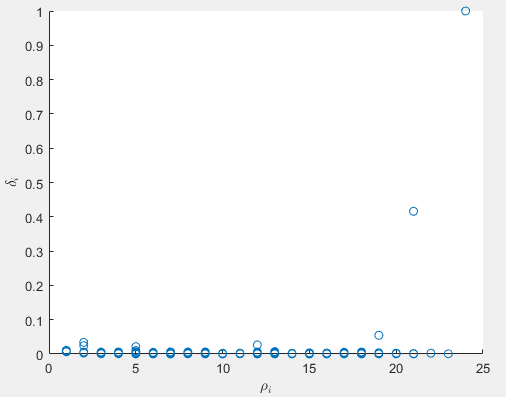
\includegraphics[scale=0.5]{seedsdensdist.png}
\end{center}
\caption{Stosunek $\rho_i$ do $\delta_i$}
\end{figure} 
\begin{figure}[h]
\centering
\begin{minipage}{.5\textwidth}
  \centering
  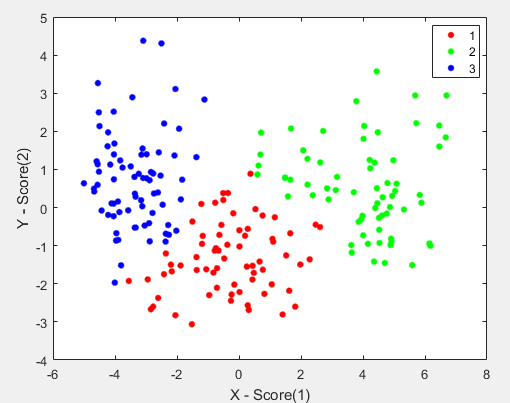
\includegraphics[width=.9\linewidth]{seedsnex.png}
  \captionof{figure}{Algorytm bez wykluczania "punktów halo"}
  \label{fig:test1}
\end{minipage}%
\begin{minipage}{.5\textwidth}
  \centering
  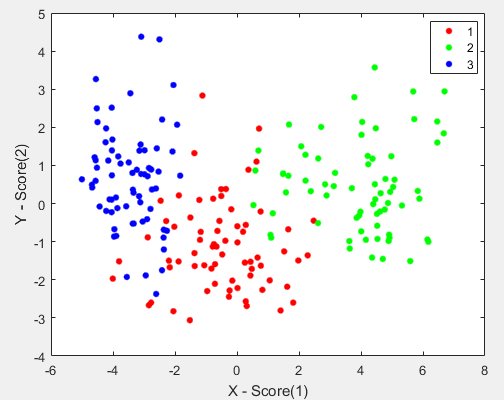
\includegraphics[width=.9\linewidth]{seedsorg.png}
  \captionof{figure}{Oryginalne klastry}
  \label{fig:test2}
\end{minipage}
\end{figure}
\newpage
\begin{figure}[h]
\centering
\begin{minipage}{.5\textwidth}
  \centering
  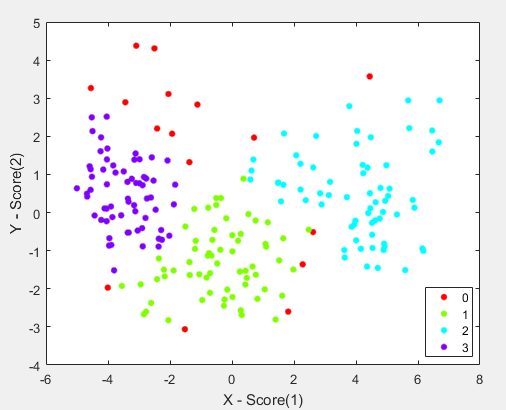
\includegraphics[width=.9\linewidth]{seedsex.png}
  \captionof{figure}{Algorytm z wykluczaniem "punktów halo"}
  \label{fig:test1}
\end{minipage}%
\begin{minipage}{.5\textwidth}
  \centering
  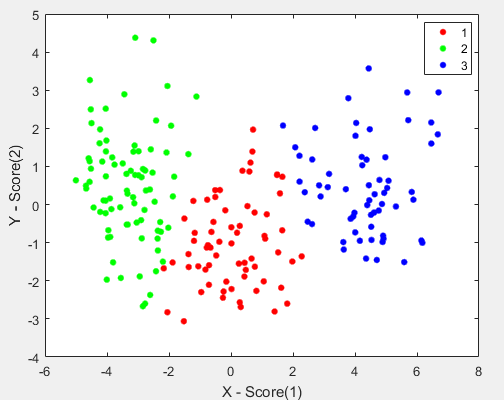
\includegraphics[width=.9\linewidth]{seedskm.png}
  \captionof{figure}{Klastry z kmeans}
  \label{fig:test2}
\end{minipage}
\end{figure}
\newpage
\subsubsection{gener}

\begin{lstlisting}[language=BASH]
mpiexec -np 4 .\ConsoleApplication1.exe gener.txt 5 0.02 50 true 4 1
\end{lstlisting}
\begin{figure}[h]
\begin{center}
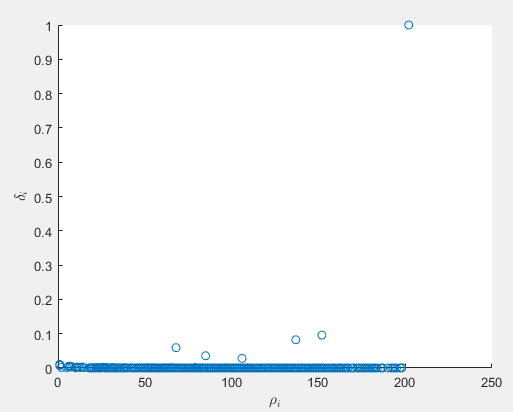
\includegraphics[scale=0.6]{generdensdist.png}
\end{center}
\caption{Stosunek $\rho_i$ do $\delta_i$}
\end{figure} 
\begin{figure}[h]
\centering
\begin{minipage}{.5\textwidth}
  \centering
  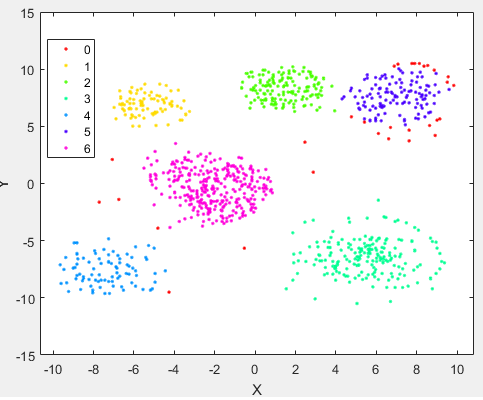
\includegraphics[width=.9\linewidth]{generex.png}
  \captionof{figure}{Algorytm z wykluczaniem "punktów halo"}
  \label{fig:test1}
\end{minipage}%
\begin{minipage}{.5\textwidth}
  \centering
  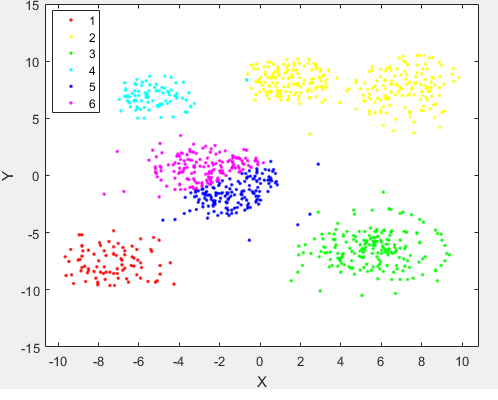
\includegraphics[width=.9\linewidth]{generkm.png}
  \captionof{figure}{Klastry z kmeans}
  \label{fig:test2}
\end{minipage}
\end{figure}
\newpage
\subsubsection{gener3}

\begin{lstlisting}[language=BASH]
mpiexec -np 4 .\ConsoleApplication1.exe gener3.txt 1.1 0.1 60
\end{lstlisting}
\begin{figure}[h]
\centering
\begin{minipage}{.5\textwidth}
  \centering
  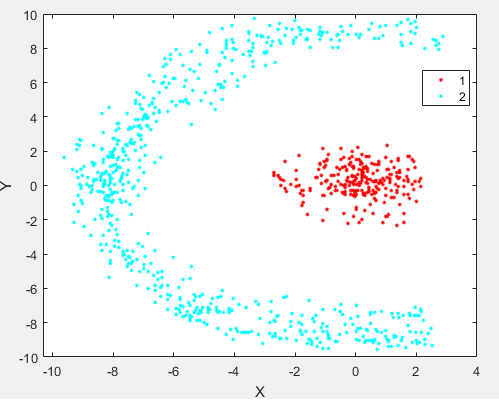
\includegraphics[width=.9\linewidth]{gener3nex.png}
  \captionof{figure}{Algorytm bez wykluczania "punktów halo"}
  \label{fig:test1}
\end{minipage}%
\begin{minipage}{.5\textwidth}
  \centering
  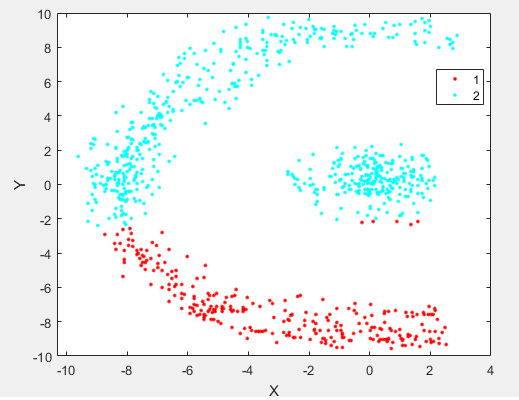
\includegraphics[width=.9\linewidth]{gener3km.png}
  \captionof{figure}{Klastry z kmeans}
  \label{fig:test2}
\end{minipage}
\end{figure}
\newpage
\subsection{Skalowalność algorytmu}
\newpage
\section{Wnioski}
\end{document}


